\chapter{Results \& Discussions}

All the published papers declared results for their experiment where the controllers were tested either for CPU or RAM utilization. They performed tests using the OFNet tool to create a vast virtual network, send large packets to the server, and use OFCProbe or OFCBench to monitor the CPU and RAM utilization via the use of SMTP messages. However, instead of OFNet, multiple instances of CBench can also be used to send those packets.

In our experiment, we have used multiple instances of CBench and Mininet. We have also used Perf to read the system utilization information directly at the server.

After having our experiment, as illustrated in the workflow depicted in Fig. \ref{workflowexperiment}, the collected raw data is represented in a graphical format. We collected and processed the system metrics such as CPU Utilization, Clock Speed, Instructions per Second, Branch mispredictions, and various level cache miss rates. These results are further discussed one by one.

\section{CPU Utilization}

Usage of the CPU refers to the use of computing power by a process or the amount of work a CPU performs. Specific tasks require massive CPU time, while others require less because of non-CPU resource requirements. A process is said to be working better if, for the same number of tasks, it utilizes less CPU.

In our result, it shows that RYU continuously utilizes less CPU than POX, depicted in Fig. \ref{CPUutilization} However, it was not such as seen in Fig. \ref{figzhu2019sdn} taken from the paper published in 2018, that depicted for at least fewer time Pox too utilize same as Ryu or even less CPU. \cite{zhu2019sdn}

\begin{figure}[!hbt]
    \centering
        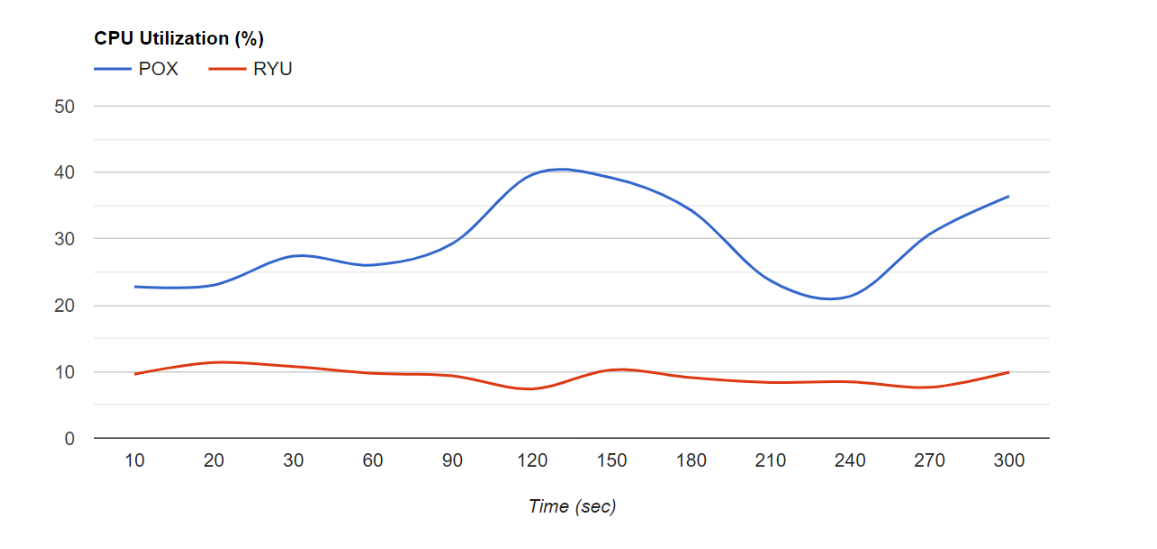
\includegraphics[width=\textwidth,keepaspectratio]{images/cpu_utilization.png}
       \caption{CPU Utilization}
        \label{CPUutilization}
\end{figure}

\section{Instructions Per Second}

Instructions per Cycle (IPC), generally referred to as clock instructions, are one component of processor performance: the total number of instructions per clock cycle.

With a specific processor, the number of instructions executed per clock is not a constant; it depends on how the individual program running communicates with the processor, and indeed the entire system, particularly the memory hierarchy. Nonetheless, certain cpu characteristics tend to contribute to designs with higher than average IPC values; the inclusion of several arithmetic logic units (an ALU is a cpu module capable of performing basic arithmetic and logical operations); and short pipelines. When evaluating various instruction sets, a simplified instruction set will contribute to a higher IPC number than applying a more complicated instruction set with the same chip technology; furthermore, with less instructions, the more complex instruction set may do more valuable work. 

\begin{figure}[!hbt]
    \centering
        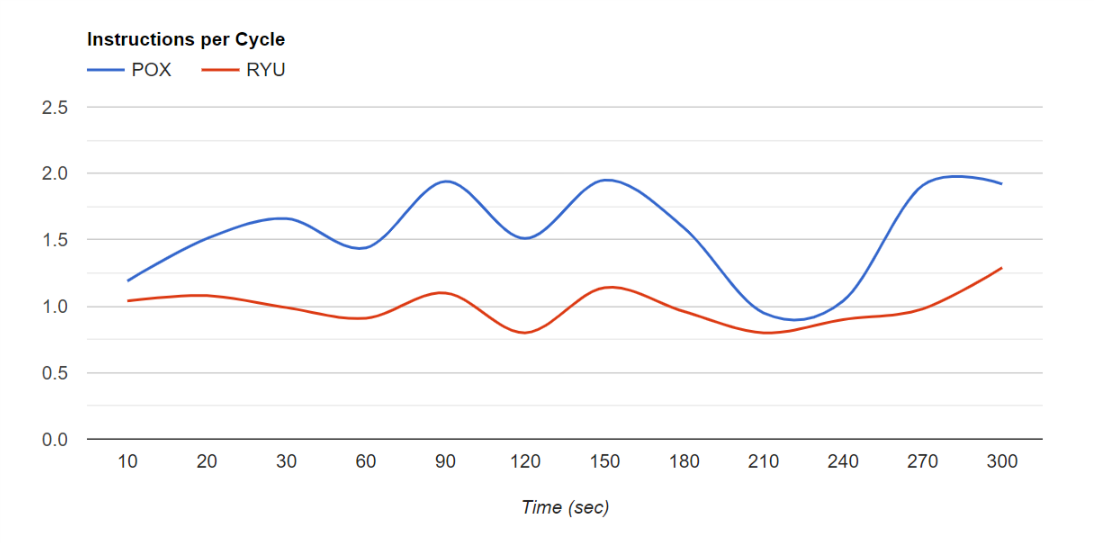
\includegraphics[width=\textwidth,keepaspectratio]{images/ipc.png}
       \caption{IPC}
        \label{ipc}
\end{figure}

The obtained result is depicted in Fig. \ref{ipc}. The effecient use of pipelining can be seen by both the controllers where both scored IPC values greater than 1. However, Pox in contrast to Ryu has better IPC.

\section{CPU Clock Speed}

CPU clock speed is calculated in Hertz — generally in gigahertz or GHz. Clock speed is a function of how many
clock cycles a Processor will execute per second. For example, a 1.8 GHz clock-rate CPU will execute 1,800,000,000 clock cycles per second. It looks so plain on the face. The more cycles a CPU can perform, the more it can do.

\begin{figure}[!hbt]
    \centering
        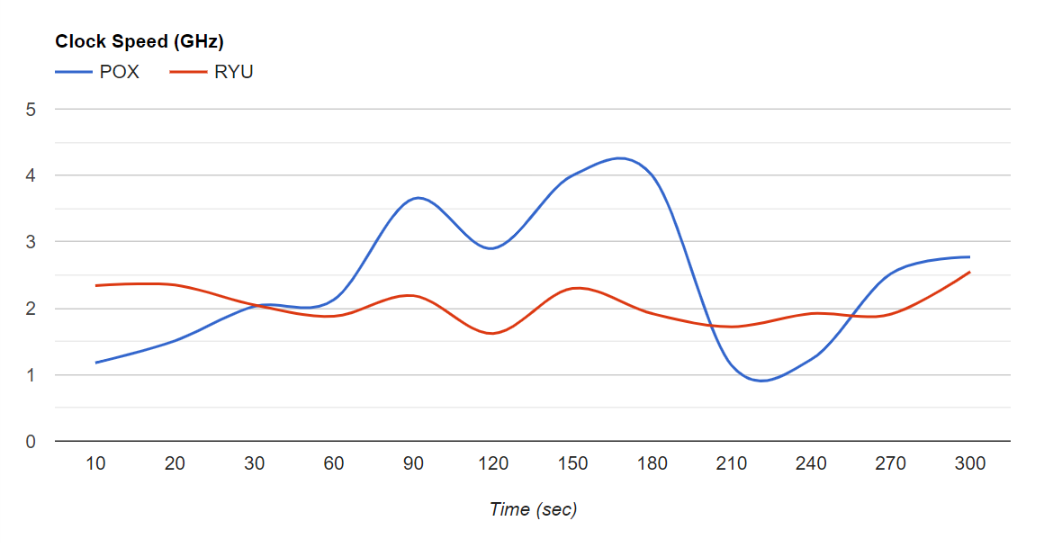
\includegraphics[width=\textwidth,keepaspectratio]{images/clock_speed.png}
       \caption{CPU Clock Speed}
        \label{clockspeed}
\end{figure}

On average both Ryu and Pox relatively has similar clock speed of about a 2GHz. However, it is also seen from Fig. \ref{clockspeed} that Pox even touches a 4GHz score or more when required. Thus, confirming that the controller uses the Turbo Boost features provided by the system used for the experiment.

\section{L1 Cache Miss Rate}



\section{L2 Cache Miss Rate}

\section{Branch Misprediction}